
\clearpage
{\Huge \flushleft Appendix}
\appendix

%%%%%%%%%%%%%%%%%%%%%%%%%%%%%%%%%%%%%%%%%%%%%%%%%%%%%%%%%%%%%%%%%%%%%%%%%%%
% CVS
%%%%%%%%%%%%%%%%%%%%%%%%%%%%%%%%%%%%%%%%%%%%%%%%%%%%%%%%%%%%%%%%%%%%%%%%%%%
\section{Appendix on Version Control with CVS}
\label{app_cvs}

Concurrent Versions System (CVS)\index{CVS!introduction} is a 
freeware version control system that is widely
used by freeware developers including those in high energy physics. 
It is used by the CERN and Fermilab computing
divisions and by the following physics collaborations: ATLAS, CMS, SDSS, NuTeV,
CLEO, and BaBar.  Now it is also being used by CDF, D0 and BTeV. 
\index{BaBar}
\index{CDF}
\index{D0}
\index{BTeV}

Additional information can be found at:

\begin{itemize}
\item CVS Documentation <http://www.fnal.gov/docs/products/cvs>
\item CVSH <http://www.fnal.gov/cd/FUE/cvsh/>      
\end{itemize}

\subsection{ The CVS Repository and Basic Concepts}
\index{CVS!introduction|(}

CVS\index{CVS!repository} extends the notion of revision control from
a collection of files in a single directory, as in CMS, to a hierarchical
collection of directories each containing revision controlled files.
For example, two CVS\index{CVS!repository} repositories designed to contain the CDF offline software
\index{CDF}
\index{CDF!repositories}
are shown in Fig.~\ref{fig_repository}.      


\begin{figure}[tbh]
\begin{center}
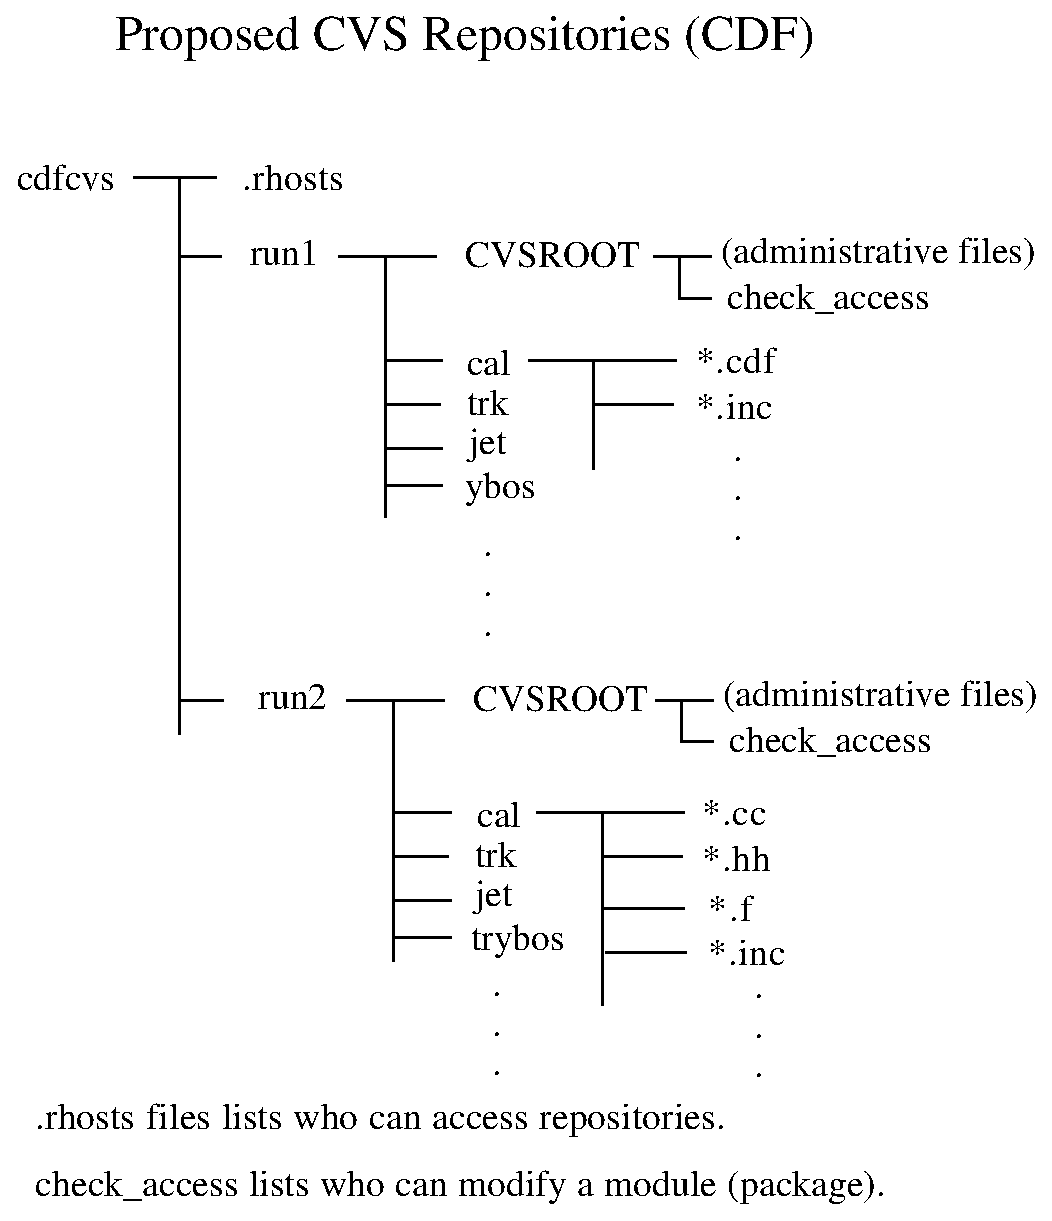
\includegraphics[width=4.0in]{two_repositories.eps}
\end{center}   

%\vspace*{-0.5in}
\caption[CVS Repositories]{
The structure of two CVS\index{CVS!repository} repositories, one for run 1 and one
for run 2.}
\label{fig_repository}
\end{figure}

Like CMS groups, CVS\index{CVS!module} collects files together into {\em modules}, and allows
operations on entire modules.  For example, the jet library would be a
module. Like a CMS class, CVS\index{CVS}
allows a collection of specific file versions to have a name, called a
{\em tag}.  CVS\index{CVS!file versions} labels each file with version
numbers, and allows branches and merging as depicted in Fig.~\ref{fig_branch}.
\begin{figure}[tbh]
\begin{center}
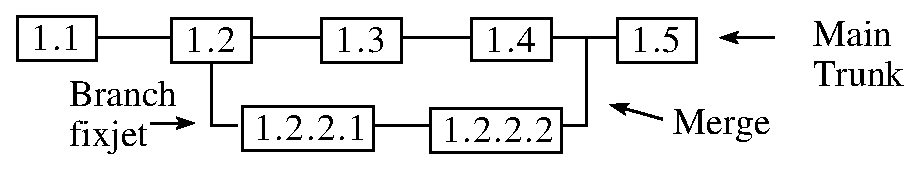
\includegraphics[width=6in]{cvs_revisions.eps}
\end{center}
\caption[Revisions, Branching and Merging]{
The versions of a particular file along the main trunk of the revision,
1.1, 1.2, 1.3, 1.4 and 1.5 are shown, along with a branch called {\ttfamily
fixjet},
that consists of modifying revision 1.2 into 1.2.2.1 and 1.2.2.2.  The
branch was merged back into the main trunk after revision 1.4 was complete,
giving revision 1.5.}
\label{fig_branch}
\end{figure}
As its name indicates, CVS\index{CVS!concurrent development} encourages concurrent revision by multiple
developers in parallel, unlike CMS which is designed for linear revision of
reserved files.  A script has been written to allow the command {\ttfamily
reserve} in CVS\index{CVS!reserve script} if desired.

\subsection{ Basic CVS Commands: A Single Revision Cycle}

As an example for the CVS\index{CVS!revision cycle} novice, the following commands perform a single
software revision cycle:
\begin{quote}
\ttfamily
cvs checkout jet/jtc90s.F\index{CVS!commands!checkout} \\
cd jet \\
cvs log jtc90s.F\index{CVS!commands!log} \\
emacs jtc90s.F \\
cvs commit -m "Changed jet energy scale!" jtc90s.F\index{CVS!commands!commit} \\
cd .. \\
cvs release -d jet \index{CVS!commands!release}\\
\end{quote}
The {\ttfamily cvs checkout}\index{CVS!commands!checkout} command creates in the users working directory a
subdirectory \texttt{jet/}, and places in \texttt{jet/} the file
\texttt{jtc90s.F}. This is like {\ttfamily CMS fetch} with an additional directory structure
created. The user goes to the \texttt{jet/} subdirectory and issues the
{\ttfamily cvs log} command\index{CVS!commands!log}, which presents her with the history of the file
\texttt{jtc90s.F}, like {\ttfamily CMS history}. The user then edits the file
(in this case using \texttt{emacs}) and places the file
back in CVS using {\ttfamily cvs commit}\index{CVS!commands!commit} and including comments, like
{\ttfamily CMS replace/keep}.  Finally the user passes back up to the working
directory and removes the entire jet/ directory tree with the command
{\ttfamily cvs release -d}\index{CVS!commands!release}, which checks to make sure there aren't any changes  
left to incorporate before deleting the files.
\index{CVS}
\index{CVS!introduction|)}

%%%%%%%%%%%%%%%%%%%%%%%%%%%%%%%%%%%%%%%%%%%%%%%%%%%%%%%%%%%%%%%%%%%%%%%%%%%
% Structure
%%%%%%%%%%%%%%%%%%%%%%%%%%%%%%%%%%%%%%%%%%%%%%%%%%%%%%%%%%%%%%%%%%%%%%%%%%%
\clearpage
\section{Appendix on the SRT Software Release Directory Structure}
\label{app_structure}

    To accommodate the storage of the various components of such a release, 
a consistent tree-structured hierarchy of directories is established. 
For expository purposes, we identify each directory with its depth (distance 
from the base) in the hierarchy. All quoted file names correspond to the 
labels in Figure~\ref{fig_directory}.

\subsection{The root directory (depth 0)}

    At the base (root) of this hierarchy is a single directory. Labelled 
``\$SRT\_DIST/'', this directory's sole purpose is to provide a starting point for 
the structure. In this root directory are entries for (the directories at the 
roots of) the two major subtrees of the structure, ``packages/''
\index{packages!area} 
 and ``releases/"\index{releases!area}. 

\subsection{The ``packages/'' directory (depth 1)}

    This directory serves as a root for the source code, documentation, 
makefiles, etc., for all versions of all packages in the product. Thus, each 
entry in ``packages/''\index{packages!area} is the starting point for a particular package. Note 
carefully that only items from the CVS\index{CVS!repository} repository are found. 

\subsubsection{Package directories ``pkgA/'', ``pkgB/'', ... (depth 2)}

    Each of these directories, direct descendents of ``packages/''
\index{packages!area} , serves as the
root of all the code, etc., associated with all versions of a single package. 
These directory names typically match the corresponding CVS\index{CVS!module} module name. Each 
such directory will have as many entries as the package has versions. 

\subsubsection{Individual version directories ``V01-00-00/", ... (depth 3)}
\label{sec_version}

    Each distinct version of a given package has its own root directory, a 
direct descendent of the package's root at depth 2 described above. The name 
of a version directory typically matches the release tag associated with the 
corresponding versions of the files in the CVS\index{CVS!tag or version} repository. 

\subsubsection{Depth 4 and beyond}
\label{sec_depth4}

    At this level, we find the source structure corresponding to (directly 
descended from the version root of) a particular version of a particular 
package. Among these entries, we might typically find: 
\begin{enumerate}
\item ``GNUmakefile'' (for the complete package)\index{packages!GNUmakefile} , 
\item  ``ups/'' (directory holding setup and unsetup files).
\index{UPS!subdirectory}
\item ``doc/'' (directory for tutorial and other documentary files), 
\item ``man/'' (directory to contain Unix-style man pages), 
\item ``src/'' (directory containing .cc and .f files), 
\item ``include/'' (directory holding .h and .inc files), 
\end{enumerate}

    Note: Figure~\ref{fig_directory} does not show all these directories, but 
they are clearly implied by the accompanying narrative. Also, 
Figure~\ref{fig_directory} labels the ``include/'' directory with the 
package name; however, this name is not a requirement of the structure but one which we 
recommend. This is because it reflects the including convention adopted in
the code: \#include pkgname/incname (see section~\ref{sec_include}).  

Recall that binary files are not intended to be located here.
However, one could conceive of additional directories here, such as ``test/'' or 
``examples/'' or ``tools/'', not necessarily part of all packages.

    The guiding principle is that, at this level, the logical structure of a 
package ought to dictate the directory structure. For reasons to become clear 
shortly, the ``include/'' directory is required, and must contain all those 
files that are visible to, and hence may be included by, any other packages or 
user software. 

The Unix-style man pages are put in the ``man/'' area of the directory 
structure. The UPS project setup file modifies the users MANPATH to include 
\index{UPS!MANPATH}
this area.

\subsection{The ``releases/'' directory (depth 1)}

    This direct descendent of the product root directory serves as a base for 
all vetted releases of the product. Each entry in this directory is the 
starting point for one such release. 

\subsubsection{Individual release directories ``1.0.0/", ... (depth 2)}

    Each of these directories, direct descendents of ``releases/", serves as the
root of all the information needed to make use of a release of the entire 
product. The name of a release directory typically matches the identification 
of a release in terms of the collection of all sources. 

    In addition, there are two standard directory names found at this level: 
``production/'' and ``current/''. These are only links to other release 
\index{soft links}
directories. They serve, however, as convenient and standardized labels so 
that users need not necessarily be cognizant of new releases: as each new 
release is installed, these directory links are intended to be broken and 
re-created as appropriate.\index{releases!soft links}

    At this level a general makefile can be created automatically to build the 
entire release tree. The makefile will simply: 
\begin{itemize}
\item invoke each of the package-specific makefiles\index{packages!GNUmakefile}  
(previously described) in turn, and 

\item install the resulting libraries and binaries into the respective 
``lib/'' and ``bin/'' flavor-specific subdirectories. 
\end{itemize}
\paragraph{\underline{Release component package directories ``pkgA/", ... (depth 3)}}

    Each of these directories corresponds to one of the 
packages\index{packages}  that make up 
the release, reflected by their parent directory, of the product. These 
directories are named for their corresponding packages. 

    However, in order to reduce unnecessary duplication of information already 
present within the ``packages/'' substructure, each of these directories is 
simply a link to the directory (at depth 3, described in 
\index{packages!soft links} 
\index{soft links}
section~\ref{sec_version} above) corresponding to the appropriate version of 
the package used to construct this release. 

\subsubsection{The ``include/'' directory (depth 3) and its descendents}
\label{sec_include}

    The intent of this directory, also a direct descendent of an individual 
release directory, is to serve as the indirect base for all .h files that 
are intended to be visible to any user of the software product. 

    This ``include/'' directory contains links, named for the individual 
\index{soft links}
\index{packages!soft links} 
packages, to the various depth 4 ``include/'' directories found under the 
``packages/'' structure (described among section~\ref{sec_depth4} above). In 
this way, code duplication is avoided, yet all include files are accessible to 
the user from one convenient source. 

The convention for including files in the source code is
 \#include pkgname/incname.
Here an 
include file, incname, is associated with a unique package, pkgname, necessary 
if two packages\index{packages!include files} have different include files with the same name.      

\subsubsection{The ``lib/'' and ``bin/'' directories (depth 3)}

    Via these directories, the remaining direct descendents of an individual 
release directory, we find a path to the software product's binaries. As is 
traditional, executables are found under ``bin/", while user-linkable libraries 
\index{linking!library locations}
are found under ``lib/". 

\subsubsection{Flavors directories ``IRIX/", ``AIX/'', ... (depth 4)}
\label{app_flavors}

\begin{sloppypar}
    These directories come into play when the software product is supported on
multiple platforms. When such is the case, ``bin/flavor/'' would serve to 
consolidate all executables for a given platform, while ``lib/flavor/'' would 
play a similar role for user-visible libraries. 
The directory is actually given a name that is a concatenation of the flavor
and version of the operating system, for example IRIX5 instead of IRIX.
This name (e.g. IRIX5) is stored in the environmental variable \$SRT\_ARCH.
\end{sloppypar}

\subsection{Usage of the directories}

    In the following sections we explain how the SRT directory structure and 
its Software Release Tools are envisioned to relate to the various client 
communities that deal with them. 

\subsubsection{A user's viewpoint}

    The UPS setup of a particular release sets the user's path, manpath, etc., 
\index{UPS!MANPATH}
\index{UPS!PATH}
in such a way that binaries are directly accessible, include files can be 
available through an environment variable pointing to the release ``include/'' 
tree, and the libraries can be used by a reference to the library tree 
environment variable via the ``-L'' compiler option. 
\index{compiler!options}

    The directory structure assumes that most users will make use of a complete
release, rather than mixing-and-matching packages across releases. If, however, 
a user would like to work with release ``A'' of a product but use version ``B'' of 
a package ``pkgC'', s/he should use the SRT ``newrel'' command to recreate the 
\index{newrel!users viewpoint}
release structure in his/her own working directory. To this command the user 
has to specify version ``B'' of package ``pkgC''. Version ``B'' of pkgC needs to 
be built in this new test release context. The user can then link his/her own 
\index{linking}
executable against this new test release. 

\begin{sloppypar}
Those users who want to write their own scripts and makefiles just need to 
know a few things. As discussed in section~\ref{sec_setup}, the UPS setup 
\index{UPS!SRT\_DIST and SRT\_CURRENT}
\index{UPS!environment}
defines the environmental variables \texttt{SRT\_DIST} and \texttt{SRT\_CURRENT}.  
The environmental variable \texttt{SRT\_ARCH} is also defined to indicate the flavor 
of operating system, as discussed in appendix~\ref{app_flavors}. In principal,
these are the only environment variables you need to use the software release 
structure. Although we strongly recommend the use of our setups and makefiles, 
the user is free to suitably define these variables to point at the right areas,
and then write their own scripts and makefiles.  The user needs to know 
that compilation with package include files\index{packages!include files}  is 
accomplished using the compilation option 
\texttt{-I\$SRT\_DIST/releases/\$SRT\_CURRENT/include}, and linking with package
\index{linking!-L option}
libraries is accomplished using the link option 
\texttt{-L\$SRT\_DIST/releases/\$SRT\_CURRENT/lib/\$SRT\_ARCH}. Users who 
prefer to do it themselves should be able to use this information to write 
their own sripts and makefiles.  However, we recommend that the provided
scripts and makefiles be used.
\end{sloppypar}

\subsubsection{A developer/contributor's viewpoint}

    In a private ``workdir'' directory, using the command ``newrel'' the developer 
\index{newrel!from developers viewpoint}
can recreate the release structure starting from a reference release. 
To modify an existing package,  the contributor can use the ``addpkg''
\index{addpkg!from developers viewpoint} command 
that checks out the module from the CVS\index{CVS!repository} repository. 
The checkout command creates the main directory structure for the package 
reflecting the module organization in CVS. Extra directories need to be 
created by the package-specific make file. The developer then 
communicates changes to the librarian, who commits them to CVS\index{CVS}.

\subsubsection{A librarian/package manager's viewpoint}

\begin{sloppypar}
    A librarian has to go through the same steps a developer goes through, but 
he has write access to the CVS\index{CVS} repository for his own 
package\index{packages!librarian}. The librarian has access to the package-specific directory in the 
\$SRT\_DIST/packages tree. This can be accomplished via a group uid, and 
trusted developers can be added or removed from this uid using the systools
commands \texttt{cmd addmember} and \texttt{cmd delmember}.
\end{sloppypar}

\subsubsection{A product/configuration manager's viewpoint}

    The product manager has write access to the entire \$SRT\_DIST tree. He can 
operate directly in the \$SRT\_DIST directories and use the ``-p'' (production) 
option of the ``newrel'' command. 
\index{newrel!managers viewpoint}

%==========================
% UPS and SRT
%==========================
\section{Appendix Using UPS with SRT}
\index{UPS}
\label{app_ups}
 
First some general comments. It is important to note that much of the 
information about which package\index{packages} 
    version works with what other package version, is contained in the release 
directory structure itself. This
    removes the requirement that this information be stored in the UPS database
\index{UPS!databases}
as dependencies. This is
\index{dependencies!UPS}
    desirable for a number of reasons. Maintaining and distributing this 
information in the form of the UPS 
    database has through the years proven to be difficult. Various recent 
additions to UPS help - cups is an
\index{UPS}
    example - but it is still true that you must be a UPS expert in order to 
\index{UPS}
effectively maintain this information. In
    a period of stable code distributions this is not a disaster; however, in a 
heavy development period it may
    become one. The other reason for minimizing UPS's knowledge of package 
\index{packages!UPS}\index{UPS}
dependencies is that it will
\index{dependencies!UPS}
    speed up and simplify the process of setting up a set of packages.
\index{packages!setup}  There 
will be fewer ambiguities about
    which versions of packages actually get setup. 

    However the concept of UPS product dependencies is still needed. There are 
\index{dependencies!UPS}
many products that we use, over
    which we have little or no control. In fact any 
package for which we do not keep
    our own CVS\index{CVS!external packages} library, would be classified in this category. Let's call 
them external packages\index{packages!external}. Examples
    would be products like cernlib or tcl/TK. These packages do not live in the 
directory structure,
    and therefore the older mechanisms for handling dependencies are still required. 
\index{UPS}
\index{dependencies!UPS}
Hopefully the coupling between
    this class of packages\index{packages!inderdependencies}  is not strong. For instance, no one would be happy if
you could only use version A of
    tcl/Tk with version B of cernlib. Also, note that references to libraries and 
binaries from this class of package are still referred to through environmental 
variables or path setting. They are not copied to the
 \verb|$SRT\_DIST/release/<version>/lib| or \verb|$SRT\_ROOT/release/<version>/bin| areas. 

\subsection{Using UPS for packages}
\index{packages!UPS} 
\index{packages!setup} 
\index{UPS!package setup}
\index{UPS}

    Packages inside the directory structure still need to be able to 
specify how environment variables,
    needed for the running of their package, must be set. For example, in the 
news product, NNTPSERVER
    must be set to the site news server machine; for tex, TEXINPUTS defines the
search list of directories to
    look for tex files. Many of the other uses of ups/setup.* files, like path 
\index{UPS}
modifying, are not needed by this type
    of package because all of the binaries live in the release structure. 
Therefore, for each
    package in the package tree, at the same level as doc, src, include and 
GNUmakefile, there is a UPS 
\index{UPS!subdirectory}
    subdirectory, which contains setup and unsetup files that are 
fragments of the
full project setup. These fragments are concatenated into the full setup 
and unsetup files in the release tree during the release build. 
Each of the fragments is a fast
equivalent of \texttt{setup <pkg>} with the appropriate version number.

\subsection{Using UPS with releases}
\index{UPS!release setup}

    In the release tree there is a UPS subdirectory at the same level as 
\index{UPS!subdirectory}
bin, lib, and include. It 
    contains a setup file that sets the path to contain the bin area of the
release and define anything else
    needed for the global release. 
From now on we refer to a global release
as a project. Thus a project is a set of experiment written products that 
get linked together into executables, and hence would form a release.  For
example online and offline could be separate projects.

The setup and unsetup file also have copied into them the 
fragments from all of the packages\index{packages!setup fragments} 
    contained in the release. These files could be built by the script that 
makes new releases\index{releases} (newrel), but currently they are build by the release 
manager by declaring the release of the project to UPS.  Marc Mengel has 
\index{UPS}
developed a utility called
\index{newrel!ups}
UPS\_COMPILE which we use to collect the fragments together into a 
\index{packages!UPS compile} 
\index{UPS!compile}
single script. The setup file
    also declares this release to the experiment UPS database so that users of 
\index{UPS!databases}
the release could say, for example, ``setup $<$project$>$ 
[$<$project-version$>$]'', as is done in section~\ref{sec_setup}.
At this time any external package dependencies could be
\index{dependencies!UPS}
defined in the UPS database.

\subsection{External Packages and UPS}
\index{packages!external} 
Not all packages used by the experiment will be included in the release 
structure. External packages, such as CERNLIB or tcl/TK or gcc, for which we 
do not usually rebuild the code, are not located in the release structure.  
They are located somewhere else which is pointed to by the normal UPS 
\index{UPS!external packages}
environmental variable.  We do not use CVS\index{CVS!external packages} to track the source code of external 
packages. There is no restriction on where the environmental variable 
\texttt{<product>\_DIR} points. If we need to rebuild external packages, we
use their own makefiles, not the SoftRelTools makefiles.

In the SoftRelTools makefiles we use the UPS \texttt{<product>\_DIR} 
\index{UPS!product variable}
environmental variables
\index{packages!external!environmental variables} 
to pickup external package libraries and include areas necessary for building.
These environmental variables may be defined through UPD dependencies, whereby
\index{dependencies!UPS}
we have declared the project to depend on a given version of an external 
package. The intent is that \texttt{<product>\_DIR} is set when we setup the
project, not via a separate ``setup $<$product$>$'' statement which might 
pickup the wrong version of the external product for the project.

%%%%%%%%%%%%%%%%%%%%%%%%%%%%%%%%%%%%%%%%%%%%%%%%%%%%%%%%%%%%%%%%%%%%%%%%%%%
% Makefiles
%%%%%%%%%%%%%%%%%%%%%%%%%%%%%%%%%%%%%%%%%%%%%%%%%%%%%%%%%%%%%%%%%%%%%%%%%%%
\section{Appendix on Makefiles in Software Release Tools}
\label{app_make}

SoftRelTools use GNU Make for building libraries and executables.
\index{gmake}
\index{gmake!GNUmakefile!user run2}
The file GNUmakefile, in the area where the gmake command
is given, tells GNU Make what to build.
%The user only needs to use
%the makefile in section~\ref{app_user_make} to link a job, and shouldn't need
%to modify it.
\index{linking}
The developer introducing a new package, or the user trying to link an
executable, needs to modify simple
makefiles described in section~\ref{app_package_make}.  Developers, code
librarians, and code managers will want to be aware of the
makefiles discussed in section~\ref{app_release_make}, but should
not need to modify them.   

\subsection{Package Makefiles}
\label{app_package_make}
\index{packages!GNUmakefile}
The following example of package makefiles, \\
\$SRT\_DIST/releases/\$SRT\_CURRENT/Framework/GNUmakefile 
and \\ \$SRT\_DIST/releases/\$SRT\_CURRENT/Framework/src/GNUmakefile, 
are used for building the libraries and executables of the Framework package.
\index{gmake}
\index{gmake!GNUmakefile!package level}
They are examples of typical package makefiles used by gmake in the examples of 
section ~\ref{sec_debug} and ~\ref{sec_newrel}. 
The first makefile only points gmake at the subdirectory src in which the
\index{gmake}
second makefile resides. The second makefile specifies the library target 
libapp.a, and includes the architecture specific makefile for the tcl package, 
on which the framework package depends.  Both makefiles include standard.mk 
which defines the compilation and dependency generation in detail.
\index{BaBar}
\begin{footnotesize}
\begin{verbatim}
$SRT\_DIST/releases/$SRT\SRT\__CURRENT/Framework/GNUmakefile 
# GNUmakefile for the BaBar Framework package
#
# uses SoftRelTools/standard.mk
#
#    Bob Jacobsen, Jan 96
#
#############################################################
# file lists (standard names, local contents)

# include file products
INC =

# library product
LIB =

#library contents
LIBFFILES  =
LIBCFILES  =
LIBCCFILES =

# subdirectories
SUBDIRS = src

# binary products
BINS =

############################################################
include SoftRelTools/standard.mk
\end{verbatim}
\end{footnotesize}
\vspace*{1in}
\begin{footnotesize}
\begin{verbatim}
$SRT_DIST/releases/current/Framework/src/GNUmakefile 
# new Makefile for Framework - the old one is unchanged.
#
# uses SoftRelTools/standard.mk
#
#############################################################
# file lists (standard names, local contents)

# include file products
INC =

# library product
LIB = libapp.a

#library contents
LIBCFILES  =
LIBCCFILES := $(shell ls *.cc)


# binary products
BINS =

# APPMain.o is required for Solaris link
all:
lib: $(libdir)/APPMain.o
$(libdir)/APPMain.o: $(libdir)/$(LIB)
        cd $(libdir); ar x $(LIB) APPMain.o
include SoftRelTools/arch_spec_Tcl.mk

############################################################
include SoftRelTools/standard.mk
\end{verbatim}
\end{footnotesize}


\subsection{Release, Standard, and Architecture Specific Makefiles}
\label{app_release_make}
At the top of every release is a GNUmakefile as shown in 
Fig.~\ref{fig_directory},~\ref{fig_dev_simple}, and ~\ref{fig_testrel}. The 
release makefile recognizes the experiment by 
means of the .experiment file, which contains names like CDF or D0. The release
\index{CDF}
\index{CDF!.experiment file}
\index{D0}
\index{D0!.experiment file}
\index{.experiment file}
makefile specifies what areas will be searched for include files when
compiling, and what areas will be searched for libraries when linking.
\index{linking}
Most important, for the library and executable targets, this file effectively 
loops over the individual package makefiles and runs make for them.
The release makefile is the heart of the building system.

The user makefiles and package makefiles described in the last section
includes the makefile standard.mk.  This makefile contains standard target 
definitions and rules for compilation and linking.  Similarly, standard.mk
\index{linking}
includes the file arch\_spec.mk, which contains the architecture specific
rules for each machine and operating system.
\clearpage

